\documentclass{beamer}

\usepackage[catalan]{babel} %text titles, etc...
\usepackage{graphicx}   %image support
\usepackage{minted}
\usepackage{array}

\usetheme{EastLansing}
\graphicspath{{../images}}

\title{\textbf{Recollida de memòria brossa}}
\author{Hash autor: 80608}
\institute[]{Facultat d'Informàtica de Barcelona - UPC\\Llenguatges de programació}
\date{Quadrimestre de tardor, 2020}

%custom commands:
\newcommand{\newSectionFrame}[1]{\section{#1} \begin{frame}\frametitle{#1}}
\newcommand{\nextSectionFrame}[1]{\begin{frame}\frametitle{#1}} 

%TODO: video entre 9 i 11 minuts. 50MB per fitxer. Resolució de 848x480 minim.


\begin{document}
    
    \frame{\titlepage}
    \begin{frame}
        \frametitle{Índex}
        \tableofcontents
    \end{frame}
    
    \newSectionFrame{Introducció als recolector de memòria brossa}
        \begin{itemize}
            \item Els \textit{garbage collectors} són un mecanisme de gestió automàtica de la memòria dinàmica d'un programa.
            \item En llenguatges sense GC, és tasca del programador gestionar les reserves de memòria dinàmica.
        \end{itemize}
    \end{frame}

    \nextSectionFrame{Introducció als recolector de memòria brossa}
        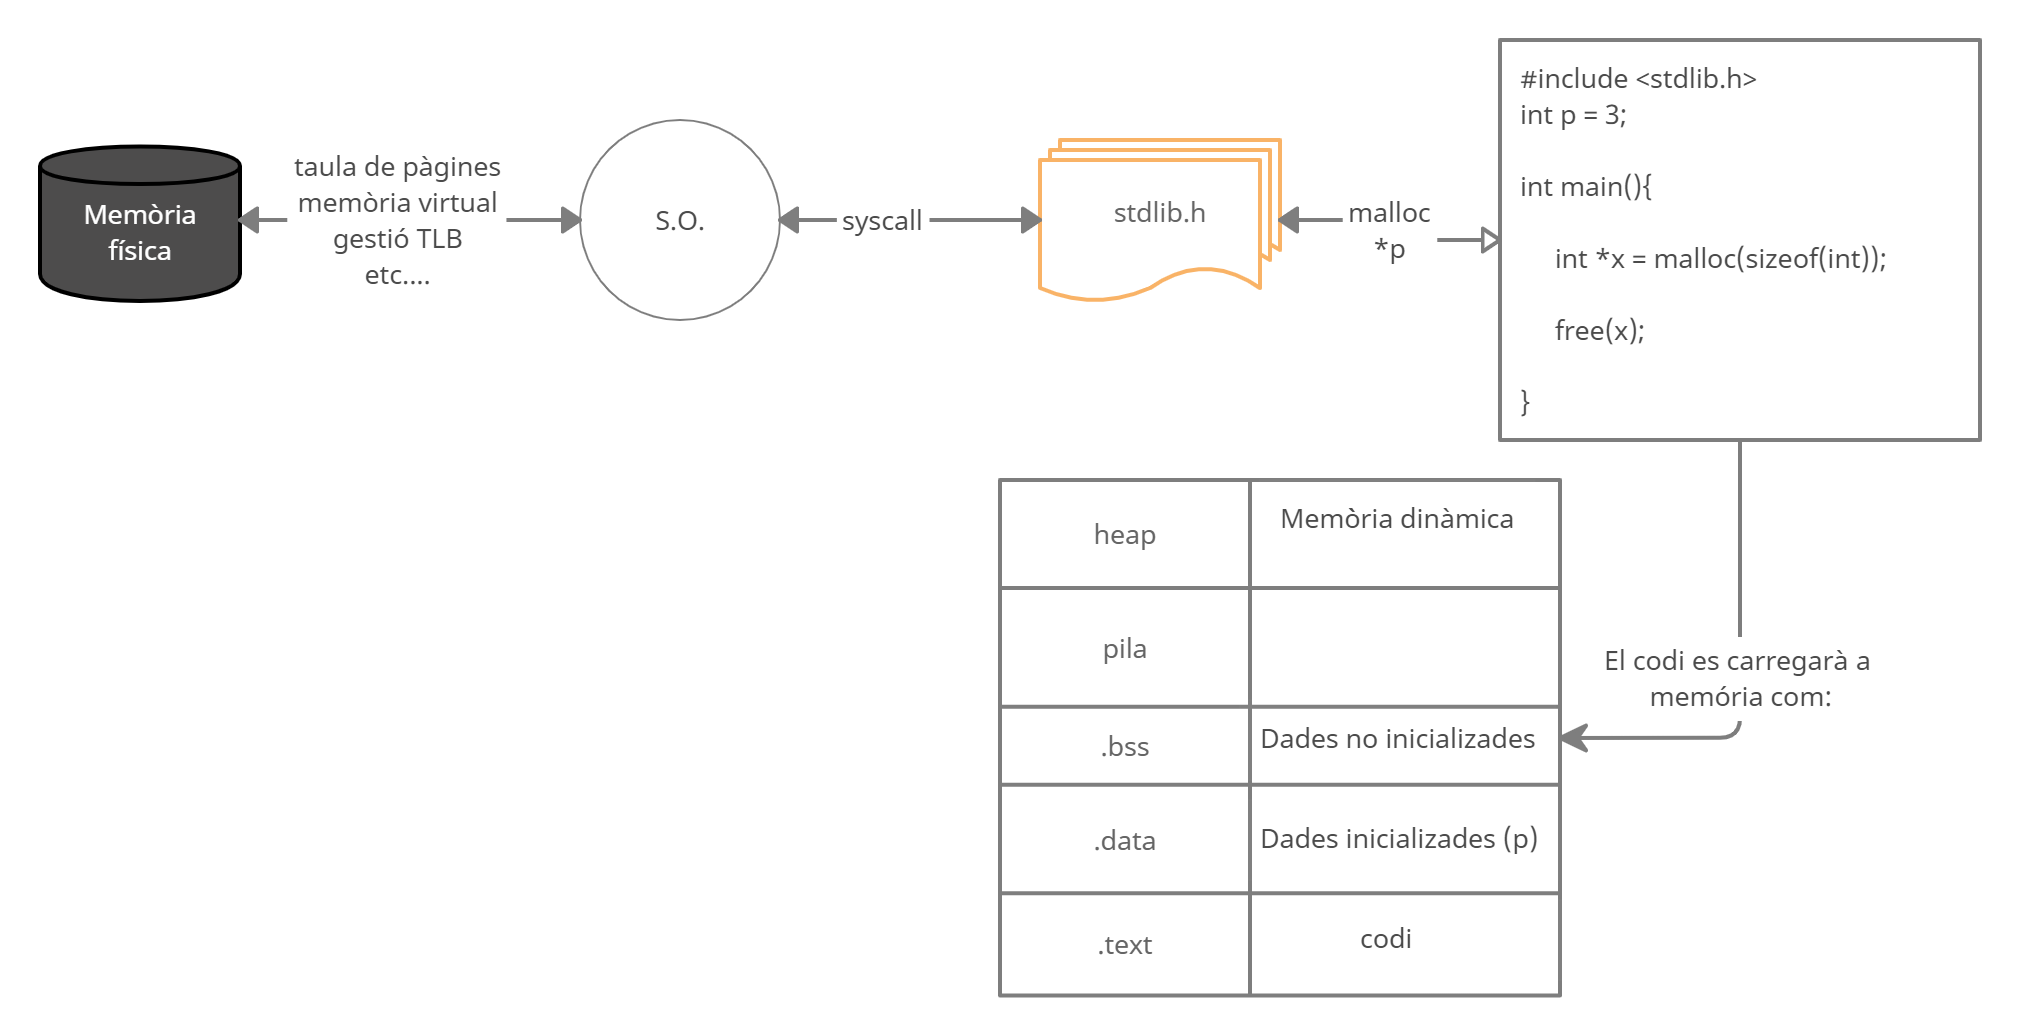
\includegraphics[width=\textwidth]{c_std_memory.png}        
    \end{frame}

    \newSectionFrame{Problemes en la gestió de la memòria}
        \begin{enumerate}
            \item Accés invàlid a memòria
            \item Fuges de memòria
            \item Reserva / alliberament incompatible
            \item Alliberar regions lliures
            \item Regions no inicializades
            \item Accés a direccions incorrectes
        \end{enumerate}
    \end{frame}

    \nextSectionFrame{Problemes en la gestió de la memòria}
        \begin{columns}
           	\column{0.5\textwidth}
			Accés invàlid a memòria
			\begin{figure}
	            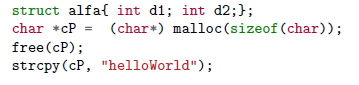
\includegraphics[width=\textwidth]{invalidAcc.png}			           
			\end{figure}

			\column{0.5\textwidth}
			Regions no inicializades
			\begin{figure}
	            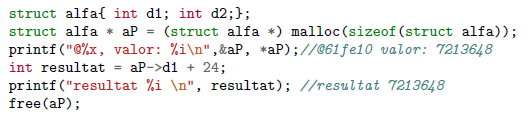
\includegraphics[width=\textwidth]{NoInicialized.png}			
			\end{figure}

        \end{columns}
    \end{frame}

    \newSectionFrame{Principis dels \textit{garbage collector}}
		Els recol·lector de memòria brossa són típics dels llenguatges O.O.
		\begin{figure}
            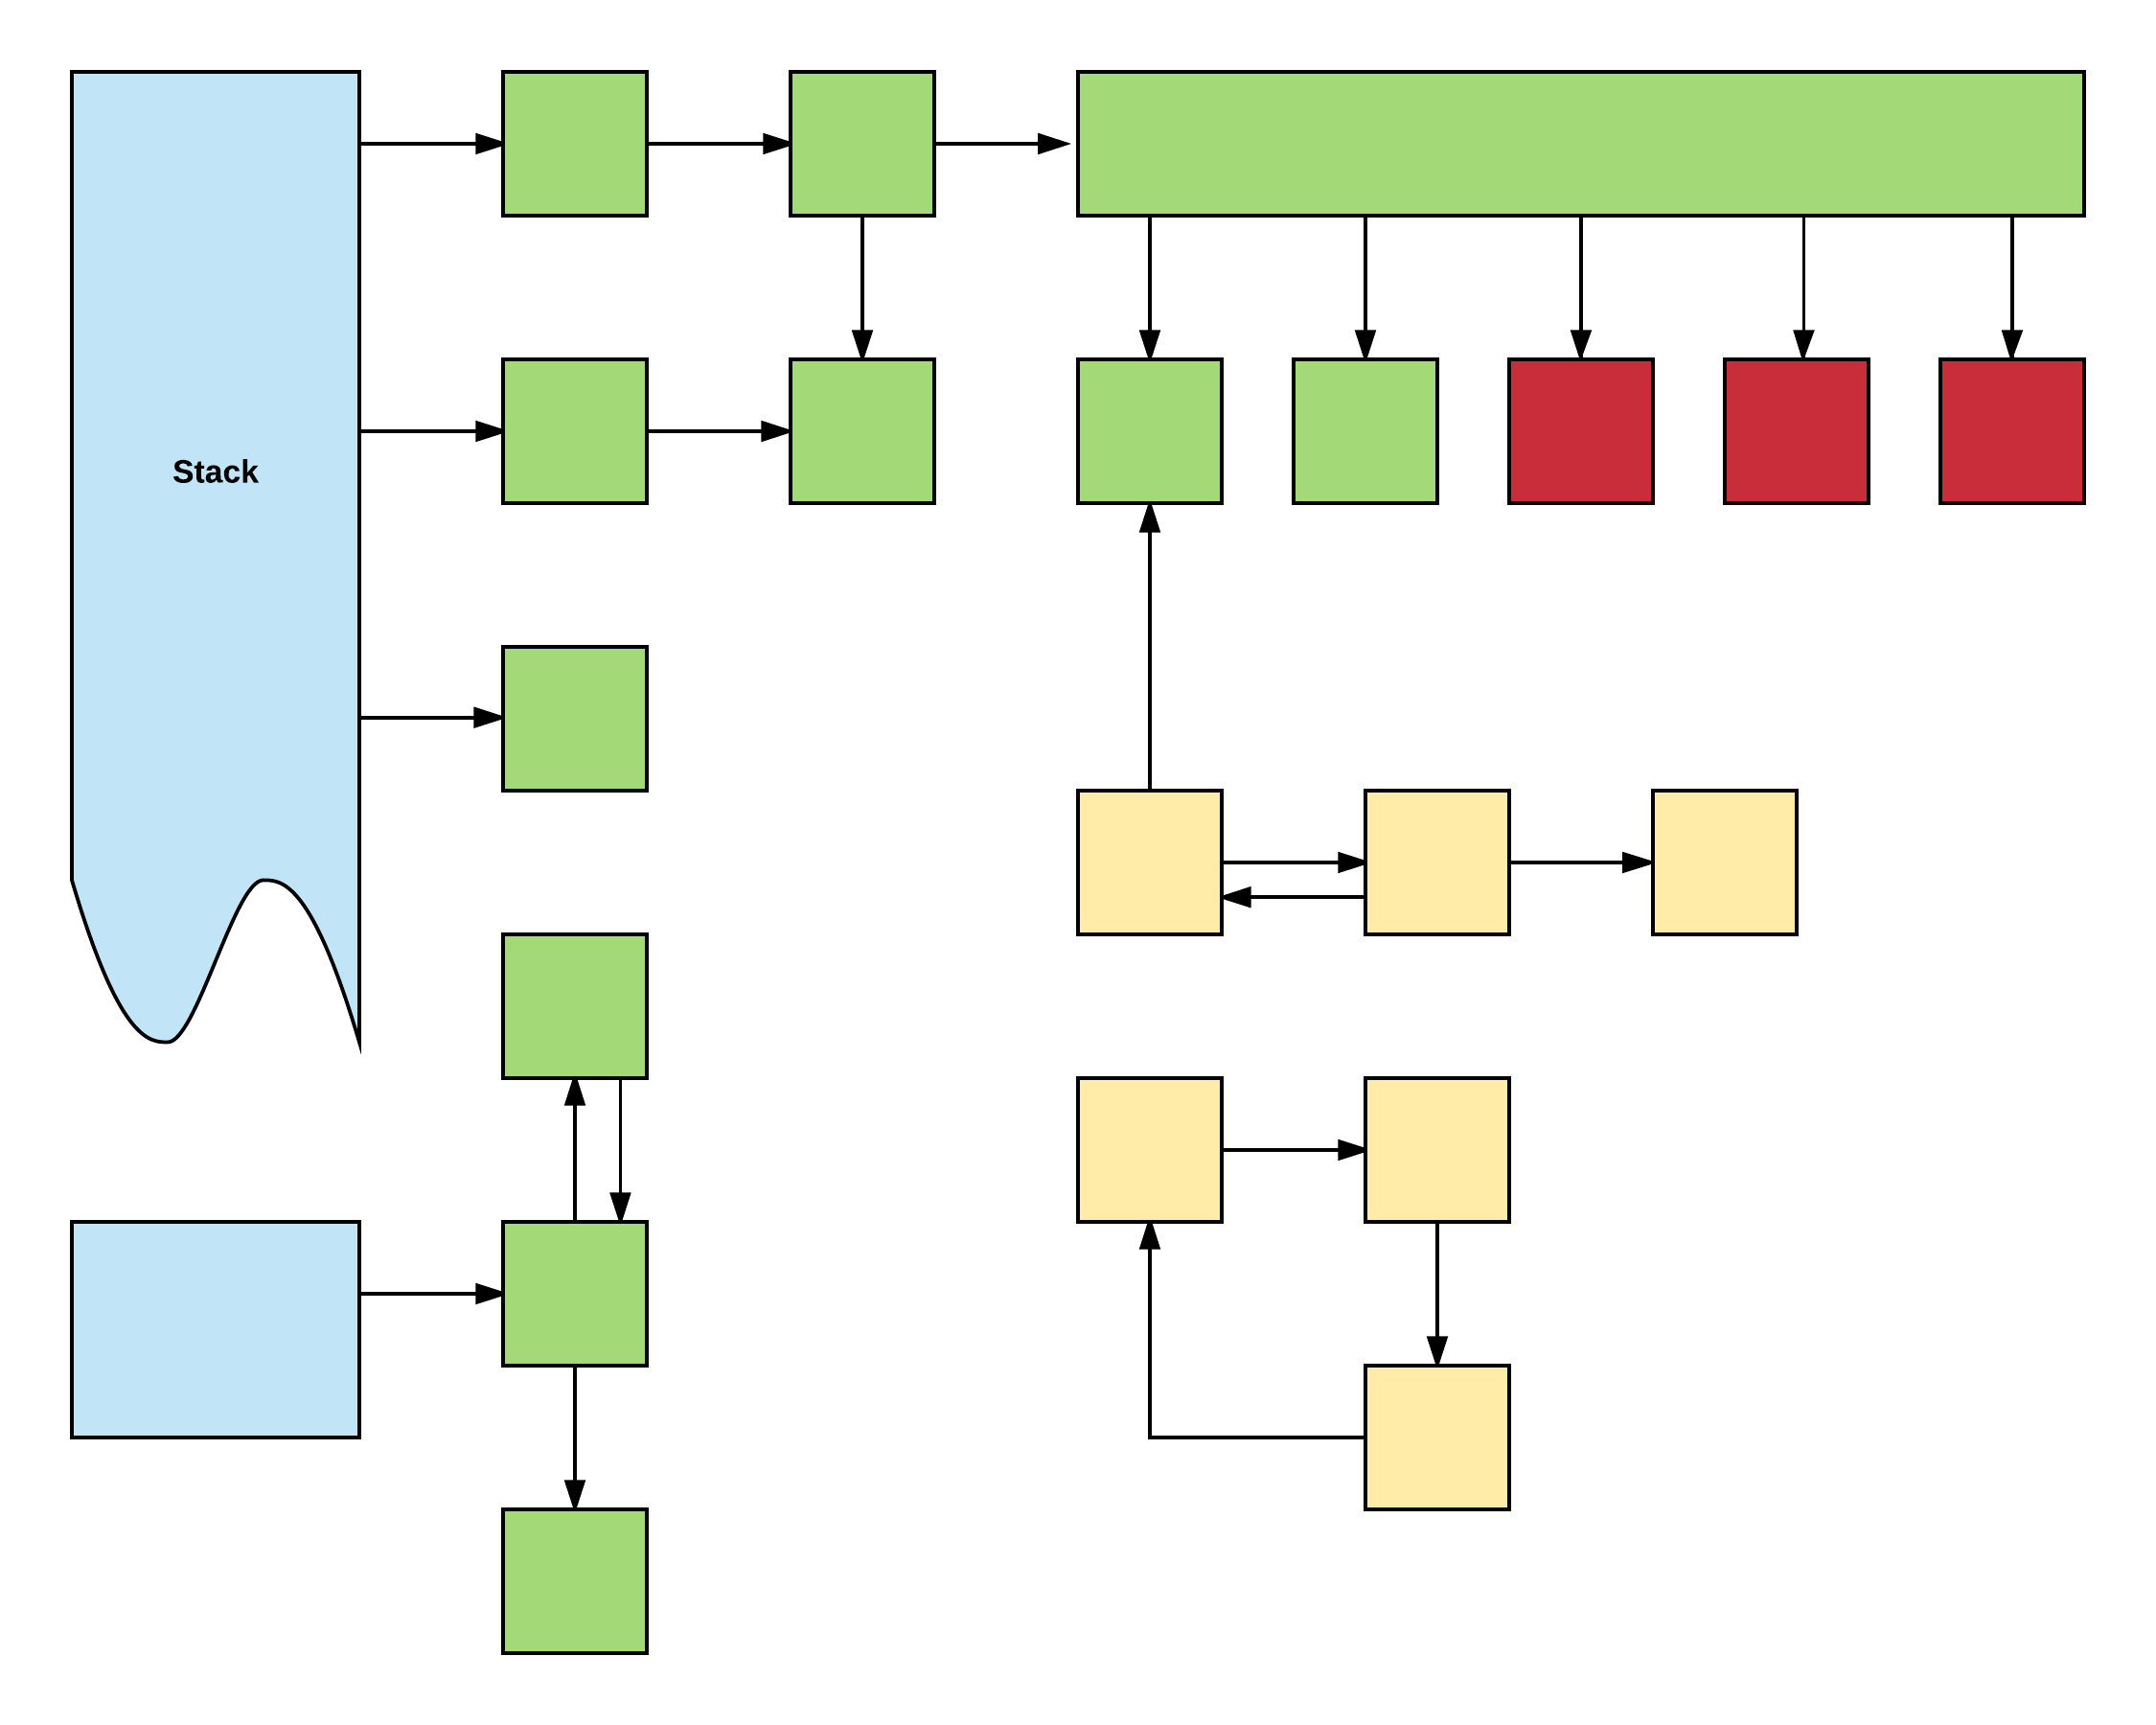
\includegraphics[scale=0.1]{memory-objects-example.png}
        \end{figure}
    \end{frame}
    
    \subsection{Objectes a Java}
    \begin{frame}
        \frametitle{Ús del GC a Java}
        A Java, les variables són apuntadors als objectes. Els objectes s'instancien amb la paraula reservada \textit{item}.
		\begin{figure}
			\centering
			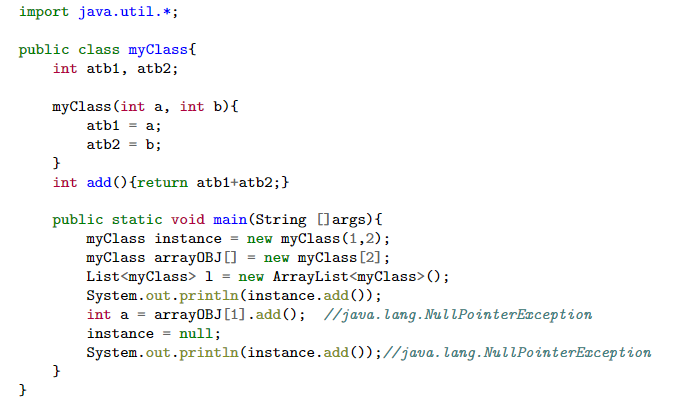
\includegraphics[height=6cm]{JavaEx1.png}
		\end{figure}        
    \end{frame}

    \subsection{Objectes a Python}
    \begin{frame}
		\frametitle{Ús del GC a Python}
		A Python, tot està representat per objectes, es poden eliminar del programa amb la crida a \textit{del}.\\
		\begin{figure}
			\centering
			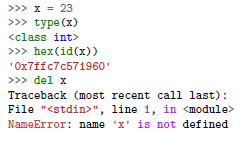
\includegraphics[scale=0.8]{pythonEx1.png}
		\end{figure}

    \end{frame}

    \newSectionFrame{Algoritmes de \textit{garbage collection}}
		Tots els algoritmes per fer recol·lecció de memòria brossa tenen el següent esquema:
		\begin{itemize}
			\item Marcar objectes
			\item Eliminar objectes 
			\item Compactar els objectes restants (si s'escau)
		\end{itemize}
		Existeixen diverses variacions d'aquest esquema, per diferents casos aplicacions.
    \end{frame}

	\newSectionFrame{\textit{Garbage collection} a Java}
		Java té diverses implementacions, totes divideixen el \textit{heap} en generacions.\\	
		Tots els objectes tenen assignat una "edad".
		\begin{figure}
			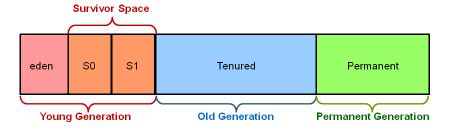
\includegraphics[scale=0.75]{JavaGenerations.png}
			\caption{Imatge extreta de Java Garbage collection basics[6]}
		\end{figure}
		\only<1>{	\begin{itemize}
			 \item \textit{Eden}: Aquí s'assignen els nous objectes. Edad = 1.
			 \item \textit{Survivor space}: Objectes no eliminats. Edad += 1.
			 \item \textit{Old generation}: Objectes supervivents. Edad $>$ Llindar.
			 \item Permanent: Objectes permanents de la JVM
				\end{itemize}
		}
		\only<2>{ \begin{itemize}
			 \item Minor GC: S'executa al omplir l'\textit{eden}.
			 \item Major GC: S'executa al omplir la \textit{old generation}.
		\end{itemize}	
		}						
	\end{frame}

	\nextSectionFrame{\textit{Garbage collection} a Java}
		\only<1>{
			A Java s'implementen a sobre aquestes particions del \textit{heap} diverses alternatives, totes elles de tipus generacionals:
			\begin{block}{Serial}
				Únic \textit{thread} per minor i major GC. Mètode esborrar i compactar.
			\end{block}
			\begin{block}{Paral·lel}
				Múltiples threads per el minor GC i opcionable al major.
			\end{block}
			\begin{block}{Concurrent Mark Sweep}
				Funciona concurrentment l'execucció del programa amb els major GC. Busca minimitzar les pauses d'execucció del programa.
			\end{block}
		}
		\only<2>{
			Desde Java JDK7, el CMS s'ha substituït per el nou algorisme G1. És un canvi de paradigma, no s'utilitza un \textit{garbage collector} generacional.
			\begin{itemize}
				\item Dividir el \textit{heap} en regions iguals.
				\item Marcar els objectes de forma paral·lela.
				\item S'eliminen primer els objects de les regions amb menys objectes (més espai de cop).
			\end{itemize}
			Molt més rendiment que el CMS.
		}
	\end{frame}

	
    \newSectionFrame{Alternatives als \textit{garbage collector}}
		\begin{columns}[onlytextwidth, t]
			\column{0.3\textwidth}
			\textbf{Assignació per frame}\\
			Consisteix en reservar memòria i descart-la sencera en un cert esdeveniment.\\
			Cal trobar aquest 'esdeveniment' i acotar la mida dels objectes.
			\column{0.3\textwidth}
			\textbf{\textit{Pool} d'objectes}\\
			Reutilitzar els objectes, cal tenir una estructura de dades per veure quins estan ocupats. Cal acotar el nombre màxim d'objectes.
			\column{0.3\textwidth}
			\textbf{Reserva directa a la pila}\\
			En alguns casos particulars, es pot reservar directament a la pila, afegint moltes restriccions als programes.
		\end{columns}
    \end{frame}

%    \newSectionFrame{Avantatges i inconvenients}
%		\frametitle{Avantatges i inconvenients GC}
%		\begin{columns}[onlytextwidth, t]
%			\column{0.5\textwidth}
%			\textbf{Avantatges}\\
%				Facilitats per programar i detectar errors.
%			\column{0.5\textwidth}
%			\textbf{Inconvenients}\\
%				Pèrdua de rendiment, aturades del programa pel GC.
%		\end{columns}
%    \end{frame}
%	
%    \begin{frame}
%		\frametitle{Avantatges i inconvenients gestó directa}
%		\begin{columns}[onlytextwidth, t]
%			\column{0.5\textwidth}
%			\textbf{Avantatges}\\
%			Ús del apuntadors i proximitat a la memòria.
%			\column{0.5\textwidth}
%			\textbf{Inconvenients}\\
%			Errors i accesos invàlids.
%		\end{columns}
%	\end{frame}
%
%	\begin{frame}
%		\frametitle{Avantatges i inconvenients \textit{frames}}
%		\begin{columns}[onlytextwidth, t]
%			\column{0.5\textwidth}
%			\textbf{Avantatges}\\
%			Més ràpid que els \textit{garbage collectors}
%			\column{0.5\textwidth}
%			\textbf{Inconvenients}\\
%			Més específic. Cal garantir una vida cíclica dels objectes i una mida %acotada.
%		\end{columns}
%	\end{frame}
%
%	\begin{frame}
%		\frametitle{Avantatges i inconvenients \textit{Pool} d'objectes}
%		\begin{columns}[onlytextwidth, t]
%			\column{0.5\textwidth}
%			\textbf{Avantatges}\\
%			Més ràpid que els \textit{garbage collectors}
%			\column{0.5\textwidth}
%			\textbf{Inconvenients}\\
%			Més específic. Cal amortitzar les reserves de memòria i definir un %màxim d'objectes (de mides similars).
%		\end{columns}
%	\end{frame}

    \newSectionFrame{Conclusions}
        \begin{columns}
            \column{0.5\textwidth}
            L'automatització de la gestió del \textit{heap} té coses a favor i en contra:
                \begin{itemize}
                    \item El rendiment i el temps de resposta baixa. 
                    \item Es facilita la programació.
                \end{itemize}
            Tenim diverses versión i configuracions de \textit{garbage collectors} a dins dels llenguatges.
            \column{0.5\textwidth}
                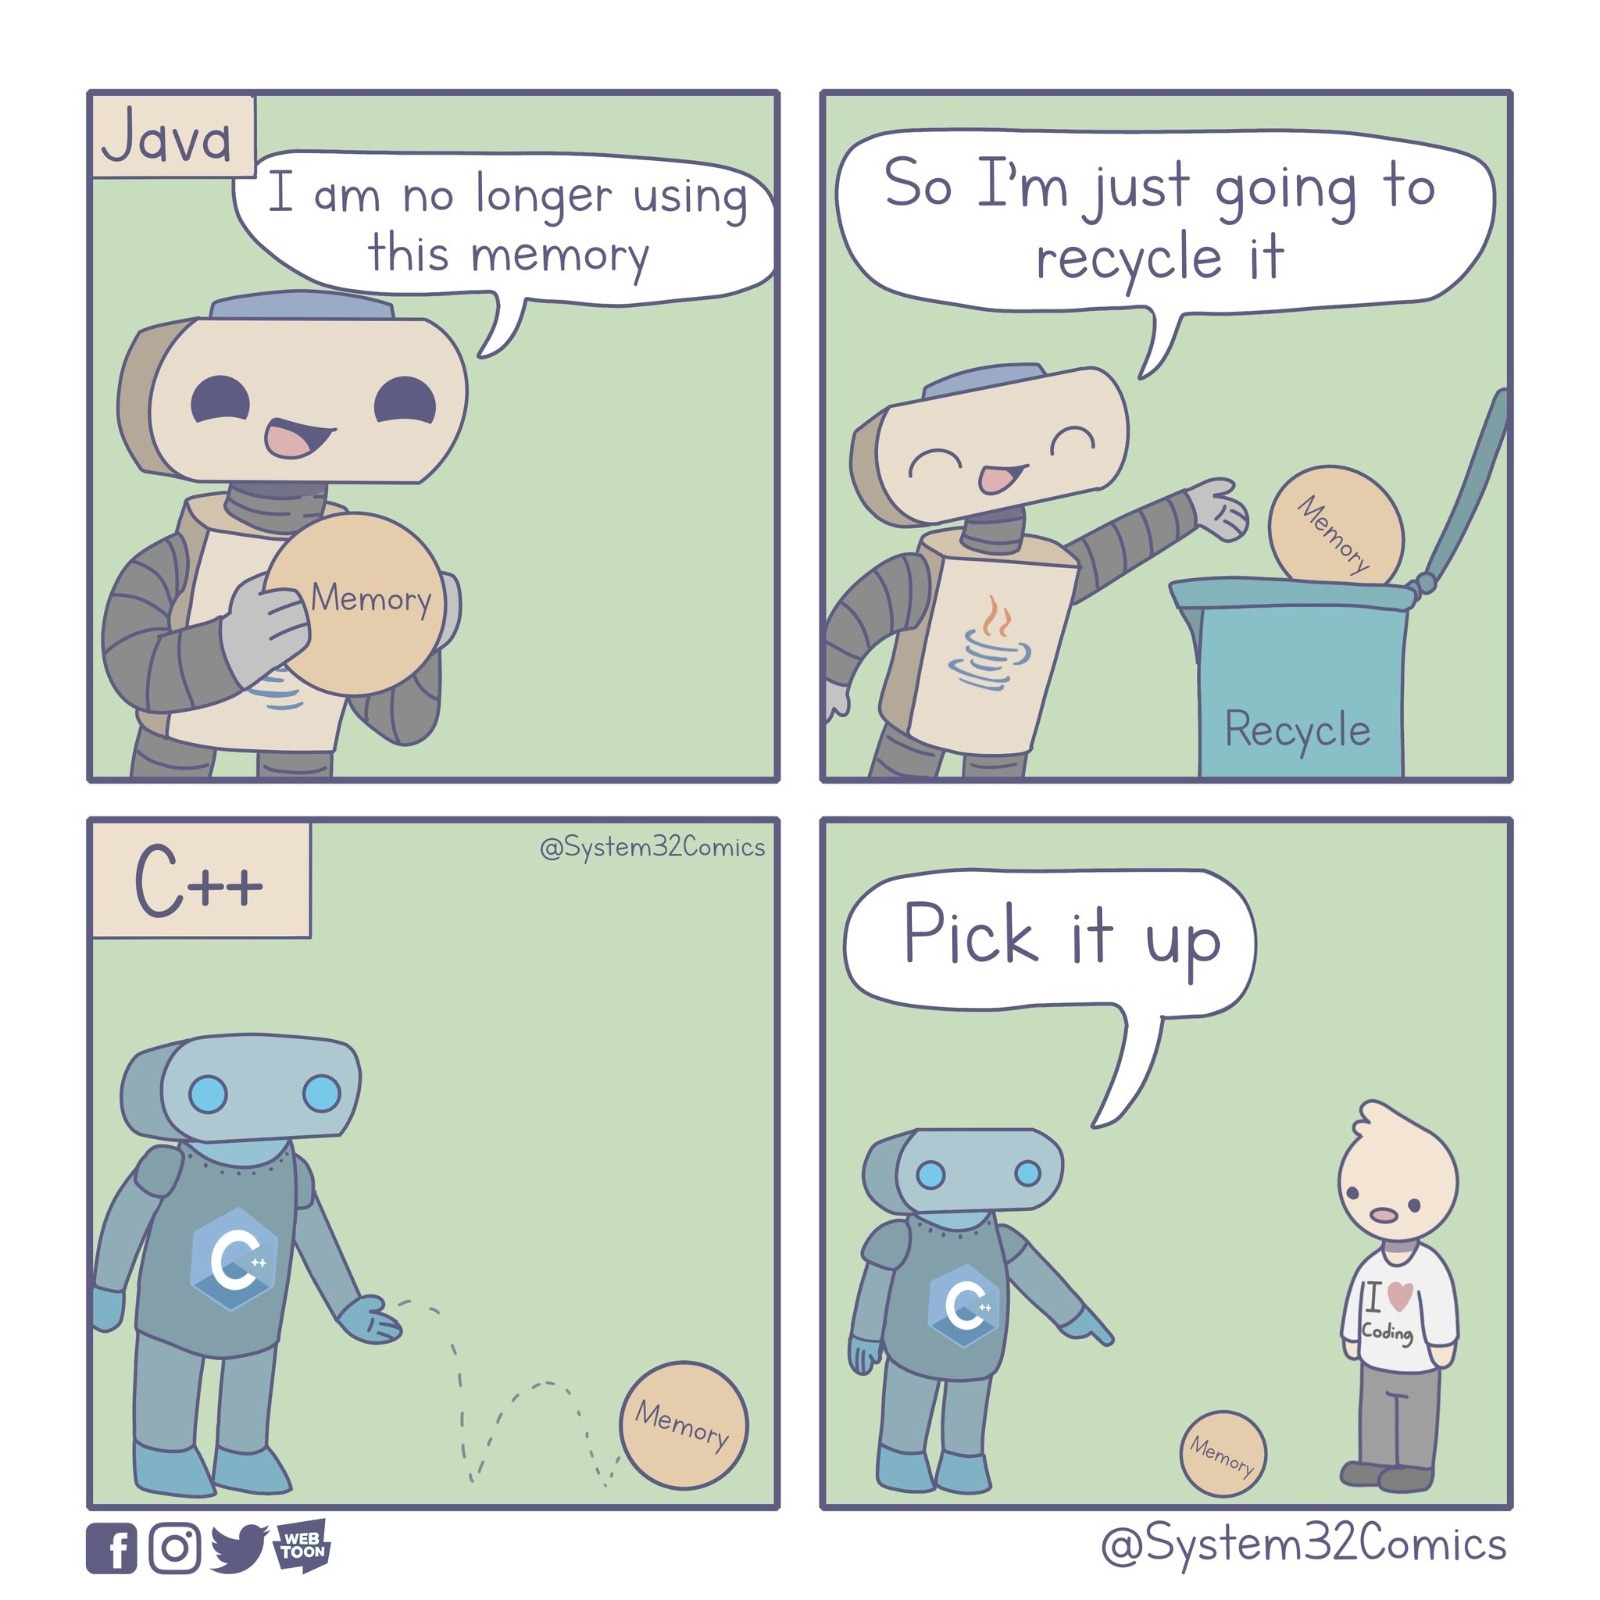
\includegraphics[width=0.8\textwidth]{Meme2.jpeg}
        \end{columns}
    \end{frame}

    \frame{\titlepage}

\end{document}
